%% LaTeX2e class for student theses
%% sections/evaluation.tex
%% 
%% Karlsruhe Institute of Technology
%% Institute for Program Structures and Data Organization
%% Chair for Software Design and Quality (SDQ)
%%
%% Dr.-Ing. Erik Burger
%% burger@kit.edu
%%
%% Version 1.3.5, 2020-06-26

\chapter{Regression}
\label{ch:Regression}

After extracting features from the elements, the next step is do learn from the data.
The goal of this Bachelor's thesis is to predict the activation barrier of a catalyst molecule.
The techniques used however are not limited to the activation barrier, 
as it can be expected that other properties of the molecule could be predicted with similar techniques.

For regression, artificial neural networks(ANNs) will be used.
Neural networks have seen a huge surge in popularity in recent years for their ability to 
adapt to high dimensional input data.
The concept is derived from biological neural networks such as the ones found in the human brain.

ANNs are a composed of a set of interconnected neurons.
Each neuron has a set of inputs $x_1 .. x_n$, a bias $b$, and an activation function $f(x)$.
The output will be the result of the activation function applied to the sum of all inputs plus the bias.

Neurons are grouped together in layers, where the output of each layer is connected to the input of the next one.
For a single prediction, the example is applied to the input layer, the network is then flooded until the output layer is reached.
In the case of regression used here, the value of the output layer is the prediction of the neural network.

% Listing 2: Tex for neural network pipeline
\begin{tikzpicture}[
    % define styles    
    init/.style={ 
         draw, 
         circle, 
         inner sep=2pt,
         font=\Huge,
         join = by -latex
    },
    squa/.style={ 
        font=\Large,
        join = by -latex
    }
]
% Top chain x1 to w1
\begin{scope}[start chain=1]
    \node[on chain=1] at (0,1.5cm)  (x1) {$x_1$};
    \node[on chain=1,join=by o-latex] (w1) {$w_1$};
\end{scope}
% Middle chain x2 to output
\begin{scope}[start chain=2]
    \node[on chain=2] (x2) {$x_2$};
    \node[on chain=2,join=by o-latex] {$w_2$};
    \node[on chain=2,init] (sigma) {$\displaystyle\Sigma$};
    \node[on chain=2,squa,label=above:{\parbox{2cm}{\centering Activation\\ function}}]   {$f_{act}$};
    \node[on chain=2,squa,label=above:Output,join=by -latex] {$y_{out}$};
\end{scope}
% Bottom chain x3 to w3
\begin{scope}[start chain=3]
    \node[on chain=3] at (0,-1.5cm) 
    (x3) {$x_3$};
    \node[on chain=3,label=below:Weights,join=by o-latex]
    (w3) {$w_3$};
\end{scope}
% Bias
\node[label=above:\parbox{2cm}{\centering Bias \\ $b$}] at (sigma|-w1) (b) {};
% Arrows joining w1, w3 and b to sigma
\draw[-latex] (w1) -- (sigma);
\draw[-latex] (w3) -- (sigma);
\draw[o-latex] (b) -- (sigma);
% left hand side brace
\draw[decorate,decoration={brace,mirror}] (x1.north west) -- node[left=10pt] {Inputs} (x3.south west);

\end{tikzpicture}


Finding a good performing network architecture is a challenging part of neural network.
Since generally no rule is known on what neural network architecture will work best on the given data, the space of possible networks needs to be explored.
A variety of choices for the network architecture can be made, such as the amount of layers, size of the layers, type of activation functions, regularization, normalization, and many more.

When choosing the network architecture, generally a bigger network will be able to adapt to the data better.
However if the network will become to big, it might encounter issues with overfitting.
Overfitting is a problem encountered when the network adapts to the training data too well.
This will decrease it's ability to generalize the data and make good predictions on previously unseen samples \ref{fig:overfitting}.

A measure to counteract overfitting is regularization.
Regularization introduces a penalty term that punishes the network for extreme values.
This causes the network to adapt less well to the training data, but in return can help with the network
performance on previously unseen data.

\begin{figure} [h]
    \centering
    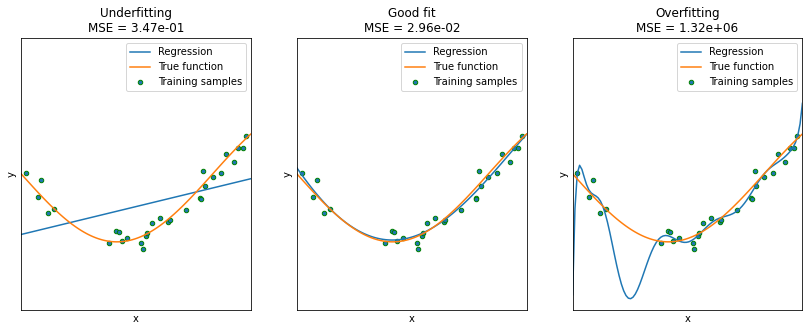
\includegraphics[width=0.9\textwidth]{figures/regression/overfitting.png} 
    \caption{Regression on a function with training examples. 
            The underfitting model is not complex enough to fit to the data well. 
            The overfitting model is too complex for the data.
            While the training error is lower for the overfitting model, 
            the overall performance of the overfitting model on previously unseen data 
            is worse than for the model with a good fit.
        }
    \label{fig:overfitting}
\end{figure}
  
To prevent overfitting while still getting good regression results, multiple network architectures need to be considered.
The networks proposed here were found by a manual exploration of the network architecture first.
In a second step, hyperparameter analysis was run to find a good network architecture.

\paragraph{Technicalities}

All networks were generated in Keras, an open-source deep learning library.
Keras offers a high level Python API to create, train and analyse neural networks.

To allow for better training and prediction results, all features and labels were standardized before being passed to the neural network.
Standardizing is a process where each feature $f$ is scaled to independently so the mean over all samples in the dataset is 0, 
and the every feature has unit variance.
This can easily be achieved by indipendently subtracting the mean $\overline{f}$ over all samples, and dividing by the standard deviation $\sigma_f$.

$$
f_{norm} = \frac{f- \overline{f}}{\sigma_f}
$$

The same scaling is applied to the labels.
This means the networks do not directly predict the activation barrier, but the networks prediction needs to be scaled back first.

Hyperparameter optimization was performed using keras-tuner, a hyperparameter tuner for Keras.
Keras tuner offerers a variety of different algorithms.
In the hyperparameter optimizations performed here, Keras Hyperband was used.
Keras Hyperband is an  implementation of the Hyperband algorithm propsed in \cite{li2017hyperband}.
It focuses on an optimized search speed compared to other Hyperparameter optimization methods, such as
Bayesian Optimization, by adaptive resource allocation and early stopping.

Hyperparameter optimization took multiple hours for LEFD features, 
and multiple days for SNAP features.
Training and hyperparameter optimization was performed on the universtiy cluster %TODO: Notwendig?
using a Nvidia Tesla V100-SXM2-32GBa GPU.

During training and hyperparameter optimization, a test set was reserved.
This test set was not used for training or validation, but only to evaluate the final performance of the networks.
All data about network performance in this chapter is measured on the test set, unless specified otherwise.

During training of a network it is common practice to reserve a validation split that is not used to train the network.
Instead, the networks performance is measured on the validation data, and tuned to achieve similar accuracies on
training and validation data.
This helps to avoid overfitting in the network, since the network can no longer just memorize the training
data, but instead has to achieve good performance on data not seen during training as well.

This means we have a total of 3 datasets, one being used for training, the other being used to validate the networks
performance during and after training, and the last being used after hyperparameter optimization to evaluate the final network
performance.

\section{Regression on fourier descriptor features}
\label{sec:Evaluation:fourier}

In the first approach, the features generated by the fourier descriptor were used to training.
Notable hyperparameters to the feature extractor here are the number of layers $l$ and the order of the fourier descriptor $o$.

The start and end height of the layers are chosen so that all the molecules in the dataset fully fit within $z_{min}$ and $z_{max}$.

The output shape of the descriptor will be an array of size $l \times (o * 4 - 1)$.
Generally, the bigger the number of fourier coefficients, the better the contour can be approximated.
However, an order that is chosen too high may increase the risk of overfitting, 
This problem is commonly referred to as "the curse of dimensionality".

A simple numerical approach to finding the order with the highest prediction accuracy is not necessarily viable in this case.
Since the ultimate goal is not to get the most accurate prediction possible, but instead discover which parts of 3d space 
are responsible for prediction, an order that offerers reasonable high accuracy without being subject too to much noise when explaining the 
prediction needs to be found. %TODO: Other reasons why order 10?

After various tests with multiple orders, an order of $k_{max} = 10$ seemed to be a good compromise between accuracy of description and accuracy of prediction.

The same problem is faced when defining the number of slices.
Here the problem becomes more tricky, since the number of slices seems to play a huge part in the architecture of the ANN used.
While the minimal number of slices should also be defined manually to allow for a proper reconstruction, the exact number of slices should be subject of a hyperparamter analysis.

%TODO: Hyperparameter analysis

Since every slice is composed of same kind of fourier coefficients, the first idea was to use convolution layers the decrease the dimensionality of the input.
Filters might be able to recognize structures in each of the slices, and applied them across the different slices.

Convolution layers heavily depend on the assumption that the relative location of features in matters.
Filter sizes were therefor chosen to correspond to the dimensions over which similarities in the structures of the features are expected.
In the case of fourier coefficients, the filter therefor were only stretched along the layer dimension, and not along the dimension of the fourier descriptors.

Multiple tests were performed with various filter sizes and convolution layers.
The regression accuracy was falling short of expectations, and the general shape of the network did not seem to change the prediction accuracy significantly.

\begin{figure} [h]
    \centering
    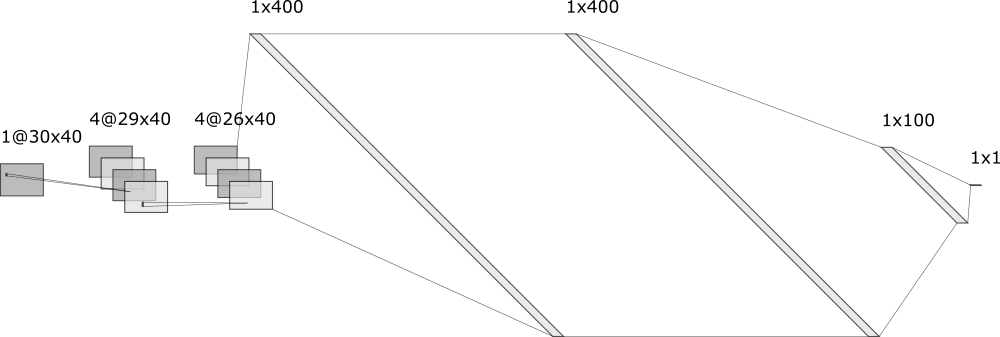
\includegraphics[width=0.7\textwidth]{figures/regression/fourier/cnn/fourier_conv_layout.png} 
    \caption{
        Architecture of the convolutional neural network used for predicting the activation barrier from fourier coefficients.
    }
    \label{fig:cnn-architecture}
\end{figure}

In first network architectures, overfitting was a mayor problem.
With regularization and other techniques the issue of overfitting could be reduced.
What became clear pretty early in the tests was that convolution layers did not improve prediction accuracy as expected.
When testing different filter configurations, the network performed best the smaller the filters got, and the fewer convolution layers were used.
In the end, the best performing Convolutional Neural Network found had two Convolution Steps with a filter size of $2 \times 1$ for the first layer, and a filter size
of $4 \times 1$ for the second layer \ref{fig:cnn-architecture}.
After the convolution layers 3 fully connected layers and the output layer followed.
Dropout and batch normalization layers were added in between to help with fighting overfitting.
The prediction accuracy of the CNN was similar yet slightly worse than the prediction accuracy achieved on autocorrelation features \cite{friederich_dos}.
The best CNN achieved a mean squared error over all test examples of $MAE=1.36$ and a coefficient of determination of $r^2=0.84$ \ref{fig:fourier_cnn}.
In comparison, the best neural network of \cite{friederich_dos} achieved a prediction accuracy of $MAE=1.12$ and $r^2=0.845$.

Since the space of possible network configurations is highly irregular, there is likely a network configuration using convolution layers 
that performs better than the one found here.
However all the tests performed were indicating that densely connected layers would achieve similar or higher accuracy.
The idea of convolution layers was therefore dropped early on, and instead the focus was shifted to optimizing a fully-connected architecture.

\begin{figure}[!htb]
    \minipage{0.1\textwidth}
    \endminipage\hfill
    \minipage{0.4\textwidth}
      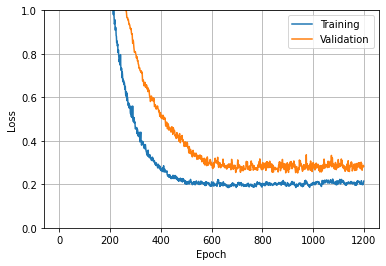
\includegraphics[width=1.0\textwidth]{figures/regression/fourier/cnn/lossCNN.png}
    \endminipage\hfill
    \minipage{0.4\textwidth}
      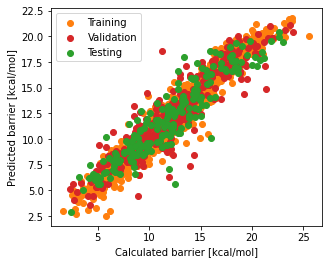
\includegraphics[width=1.0\textwidth]{figures/regression/fourier/cnn/scatterCNN.png}
    \endminipage\hfill
    \minipage{0.1\textwidth}
    \endminipage
    \caption{
        Loss while training the CNN. The jitter in the training loss during convergence is likely caused by the dropout layers. 
        The optimization goal was minimizing the mean squared error. 
        Training was performed on 80\% of the data.
        On the right are the predictions of the activation barrier in comparison to the real values ($MAE=1.36$, $r^2=0.84$).
    }
    \label{fig:fourier_cnn}
\end{figure}

Since previous research has proven that similar accuracy to the convolution approach can be achieved by learning from autocorrelation features,
the next idea was to use a transfer learning approach.
In a first step, the network would be taught to predict the autocorrelation features computed in \cite{friederich_dos}.
In a second step, the network is then extended to learn to predict that activation barrier \ref{fig:transferlearn}.
The hope was that teaching the network about autocorrelation features, the model would learn to recognize relevant properties of a catalyst.
In a second step, the entire network would then be trained to adapt specifically to the activation barrier.

\begin{figure} [h]
    \centering
    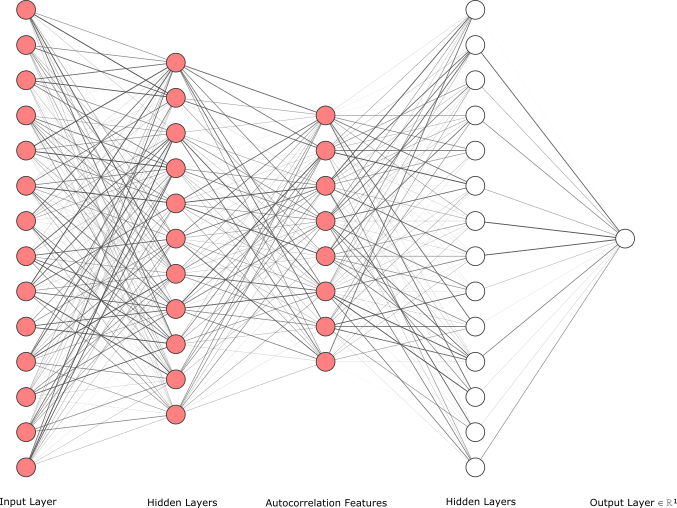
\includegraphics[width=0.7\textwidth]{figures/regression/fourier/nn.png} 
    \caption{Illustration of the transfer learning approach.
        In red the original model predicting autocorrelation features from the input is illustrated.
        In white the second part of the network, predicting the activation barrier from the autocorrelation features, is illustrated.
        Different sizes and amounts of hidden layers were tested. Here, single hidden layers are shown for illustration purposes.
    }
    \label{fig:transferlearn}
\end{figure}

Since the convolutional approach did not seem to improve results, a fully connected architecture predicting autocorrelation features from fourier coefficients 
was used.
Since there were 30 autocorrelation features used, the last layer of the network had a size of 30.
Findings about good hyperparameter, such as layer size, regularization and dropout rates, could be partly reused from the convolution step.
In the end, a network that predicted 30 independent autocorrelation features was found.
The network was able to predict some autocorrelation with very high accuracy. Specifically, the $T$ features and $I$ features were
predicted with an accuracy of $r^2 > 0.98$. 
Other features, such as $Z$ features, were lacking behind in accuracy, with the network only being able to reach accuracy of $r^2<0.96$ for some features.
The features the network was able to approximate well were also less important to the network found in \cite{friederich_dos}, while the features 
the network performed poorly on were the more important features \ref{fig:transfer_result}.

\begin{figure}[!htb]
    \minipage{0.32\textwidth}
      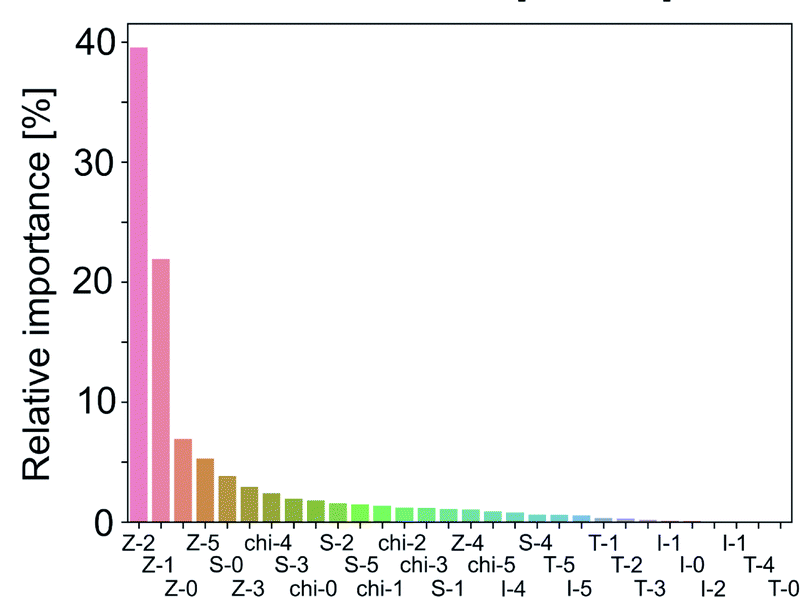
\includegraphics[width=1.0\textwidth]{figures/regression/fourier/importance_map.png}
    \endminipage\hfill
    \minipage{0.32\textwidth}
      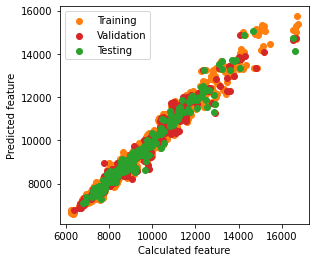
\includegraphics[width=1.0\textwidth]{figures/regression/fourier/transfer/scatterZ2.png}
    \endminipage
    \minipage{0.32\textwidth}
      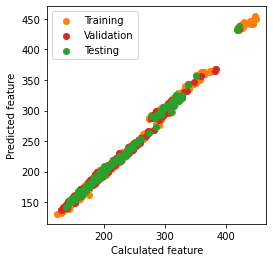
\includegraphics[width=1.0\textwidth]{figures/regression/fourier/transfer/scatterT0.png}
    \endminipage
    \caption{
    Left: Importance of features for the neural networks discussed in \cite{friederich_dos}.
    Middle: Prediction of Z-2 features from fourier features.
    Right: Prediction of T-0 features from fourier features. 
    The network was trained on 80\% of the data points.
    }
    \label{fig:transfer_result}
\end{figure}

After the network predicting the autocorrelation features was trained, the the transfer learning was started.
The last layers of model were removed, and replaced with newly initialized layers.
These newly added layers have and output size of 1 to allow for prediction of the activation barrier.
The best configuration found kept the first 3 layers of the original network, and then added 3 additional hidden layers and one output layer.
Regularization and normalization was used for some of the layers.
The model was then trained again with fourier coefficients as input and activation barriers as output.
Compared the convolution approach, the network took longer to converge, the overall regression accuracy improved.
The network achieved a $r^2=0.874$ and a $MAE=1.139$ when trained on 80\% of the data \ref{fig:transfer_final}.

\begin{figure}[!htb]
    \minipage{0.3333\textwidth}
      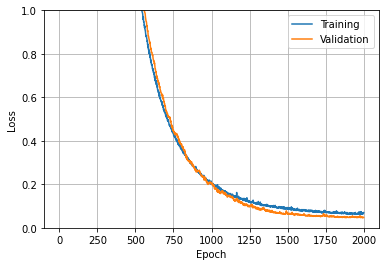
\includegraphics[width=1.0\textwidth]{figures/regression/fourier/transfer/lossTransferAutocor.png}
    \endminipage\hfill
    \minipage{0.3333\textwidth}
      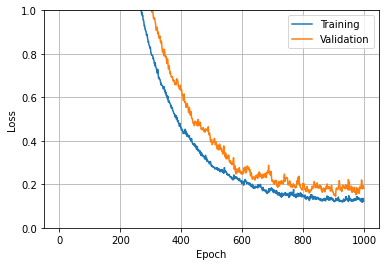
\includegraphics[width=1.0\textwidth]{figures/regression/fourier/transfer/lossTransferFull.png}
    \endminipage\hfill
    \minipage{0.3333\textwidth}
      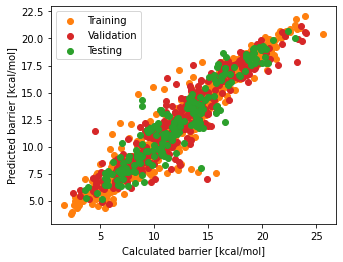
\includegraphics[width=1.0\textwidth]{figures/regression/fourier/transfer/scatterTransferFull.png}
    \endminipage
    \caption{
    Loss of the network being trained to predict autocorrelation features (right).
    The adapted network is then trained again to predict the activation barrier. The loss function in the middle shows the second training.
    The prediction accuracy has slight improved (right).  
    }
    \label{fig:transfer_final}
\end{figure}

In an attempt to find a better network architecture, a hyperparameter optimization was performed.
Hyperparameter optimization is a way of finding good hyperparameter for the underlying problem.
A searchspace need to be defined manually first, an optimization algorithm is then run to find good parameters within the search space.
Generally a bigger search space mean longer computation time for the hyperparameter algorithm.
The search space here was limited by the findings of manual hyperparamter tuning.
Notable optimization values given to the hyperparamter tuner were the number of convolution layers, 
the number and size of fully connected layers, the regularization rate of these layers, and the dropout rate for the layers.


\begin{figure}[!htb]
    \minipage{0.3333\textwidth}
      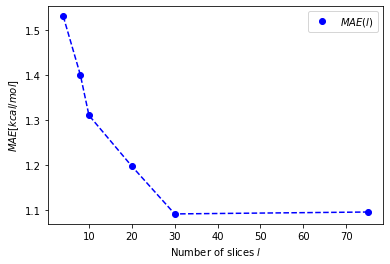
\includegraphics[width=1.0\textwidth]{figures/regression/fourier/mae_layer.png}
    \endminipage\hfill
    \minipage{0.3333\textwidth}
      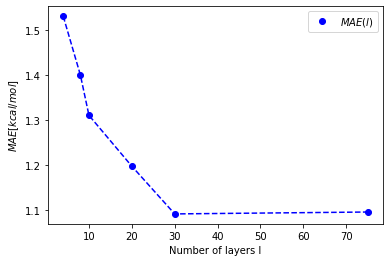
\includegraphics[width=1.0\textwidth]{figures/regression/fourier/r2_layer.png}
    \endminipage\hfill
    \minipage{0.3333\textwidth}
      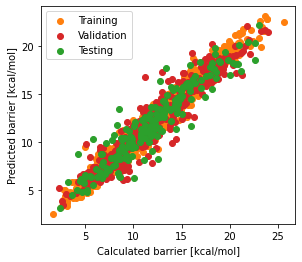
\includegraphics[width=1.0\textwidth]{figures/regression/fourier/scatterHyperparam.png}
    \endminipage
    \caption{
    The $r^2$ values and $MAE$ for different layer heights.
    For all layer heights a separate hyperparameter optimization wa run, resulting in different network architectures.
    All networks are trained using 80\% on the data. The $r^2$ scores and $MAE$ were evaluated later using a test dataset.
    The on the right the prediction of the best performing network found in the hyperparameter optimization step is plotted.
    The best network was found using a input layer height of $0.2 \AA$ resulting in $75$ layers. 
    The $MAE=1.096$ and $r^2=0.882$ are the highest accuracy so far.
    }
    \label{fig:fourier_final}
\end{figure}


In addition, multiple hyperparameter optimizations were performed for different layer heights $l$.
Since the layer heigh also changes the input size of the neural network, an assumption about the 
architecture across different layer heights is not feasible.
For ever layer height a separate hyperparamter optimization was run \ref{fig:fourier_final}.
The best hyperparameters found for every input site vary substantially.

After a certain layer height the prediction accuracy seems to no longer improve.
The step from 30 to 75 layers does not change the accuracy significancy, while more than doubling input size.
The small improvement in accuracy from 30 to 75 layers might not necessarily mean a higher overall classification accuracy of the network,
but could also be to randomness when selecting training and test examples or randomness during training.

The process shows that performing regression on fourier features is possible.
The accuracy however is not significantly higher than the accuracy achieved on graph convolutions.
Since the goal of this thesis is to learn from the 3D structure of the molecule, the similar performance 
indicates that the information learned from the 3d structure is limited.
This assumption is further validated by the fact that the transfer learning approach that 
basically eliminates spacial information about the network in the middle of the network, achieves similar accuracy to the 
network trained on features that do not include any information about the 3d structure.

Due to these results, a different feature extractor, SNAP, was developed.

\section{Regression on SNAP features}
\label{sec:Evaluation:snap}

Similar to the feature space for fourier coefficients, the size of the SNAP feature space is determined by two factors.
The first is the number of elements in the dataset.
The second is the resolution of the encoding for each type of element, defined by $n_{max}$ and $l_{max}$.

Other hyperparameters, such as the choice of radial basis functions, might influence the prediction accuracy further.

The number of radial basis functions $n_{max}$ and the maximum degree of spherical harmonics $l_{max}$ do both influence
the input dimension.
The ideal network architecture for different values will therefor vary too.
Since the values determine the accuracy with which accuracy the space is encoded, choosing these values purely 
based on which combination achieves the highest classification accuracy is not feasible.
The higher the degree of the spherical harmonics and radial basis functions, the more precise the element can be described.
The higher number of coefficients might however come at the price of noise when trying to explain the prediction later on.
A good balance between interpretability and accuracy was found with $l_{max}=n_{max}=3$. %TODO: Really? 

Hyperparameter analysis was performed on different combinations of $n_{max}$, $l_{max}$.
Since hyperparameter optimization is very computationally expensive, taking up to multiple days on modern high-performance 
server hardware, the number of combinations that could be explored is limited.

SNAP features are not fully rotationally invariant.
In order to allow the model to learn about the different possible rotations of the molecule, data augmentation was used.
In the hyperparameter optimizations performed here, 20 evenly spaced rotations of the molecule along the $z$-Axis were used.
The features for all of the 20 rotations was then fed into the model.
Tests with different augmentation steps showed that 20 augmentations seemed to be a good balance between 
accuracy and training speed.
Since the size of training examples rises linearly with the number of data augmentations,
high numbers of augmentations will drastically decrease training speeds.
This will in effect also reduce the speed of hyperparameter optimization.

\subsection{Convolutional Neural Network}

Similar to the features generated by EFD, the output of SNAP can be shaped into a feature matrix again.
Here, each layer will correspond to one species of atoms.
Since the dataset the model is trained on consists of 12 different species of atoms, the feature matrix will have a height of 12.
Each row will then hold the coefficients describing the density of this species around the iridium center.
Depending on the choice of $n_{max}$ and $l_{max}$, the number of coefficients will change.

Since a coefficient of the $k$-th row will correspond to $c^k_{nlm}$, meaning every coefficient in the same colum has the same spacial meaning,
a convolutional neural network was the first idea to reduce the size of the input space and allow the network to learn structure in the input data.

Since not every molecule in the dataset consists of every atom, the input matrix will generally be sparse.
Rows that correspond to atoms not in the dataset will be filled with 0.
A filter that learns the general structure of the space and that is moved over the different species, therefor 
being able to ignore sparse inputs seemed to be a good choice.

Using a hyperparameter optimization to find the ideal filter size and number of convolution layers however showed
the a fully connected approach reaches higher accuracy than convolutional layers.
The hyperparameter optimizer not only gravitated towards a small amount of filters, but also towards 
the smallest possible filter size allowed in the hyperparameter space.

In further optimization the idea of convolution layers was therefor dropped in favour of fully connected layers.

\subsection{Fully connected neural network}

In a next step, hyperparameter optimization was focused on fully connected layers.
For different combinations of $n_{max}$ and $l_{max}$ hyperparameter optimizations were run.

The hyperparameter optimizer was allowed to choose between 1 to 6 hidden layers.
For each layer, the number of neurons, regularization rate and dropout rate could be chosen by the optimizer.
Additionally, the optimizer had the option to add a batch normalization layer after each of the layers.
The layers were then finished off with one neuron fully connected to the last hidden layer.

The activation function for each of the layer was fixed to Relu activations.

Hyperparameter analysis was then run using Keras Hyperband tuner.
Keras Hyperband is an  implementation of the Hyperband algorithm propsed in \cite{li2017hyperband}.
Hyperband focuses on an optimized search speed compared to other Hyperparameter optimization methods, such as
Bayesian Optimization. %TODO: Mehr?

Using the Hyperband Optimizer, the configurations discussed in the following sections were found.
Since the hyperparameter space was limited, for example to the use of relu activation functions,
the best performing models were then further enhanced manually.

\paragraph{Feature size}
The expectation was that the more accurate the density space would be described, the higher the prediction accuracy would be.
However after a full hyperparameter optimization on a variety of combinations of $n_{max}$ and $l_{max}$,
the differences in accuracy were not as significant as expected.
While increasing the number of $n_{max}$ coefficients seemed to increase the prediction accuracy,
overall the randoms of the training process seemed to have far higher influence on the models performance.
The infleunce of $n_{max}$ seemed to dominate over the influence of $l_{max}$.
Highest prediction accuracies where achieved by networks performing regression on features generated with $n_{max} > 6$.

Since hyperparameter searches for are very costly, taking up multiple days on modern day cloud-computing hardware,
hyperparameter analysis was run to an $l_{max} = 9$.
Significantly increasing $n_{max}$ might further improve prediction accuracy.

%TODO: Redo with actual values
\begin{figure}[!htb]
  \minipage{0.3333\textwidth}
    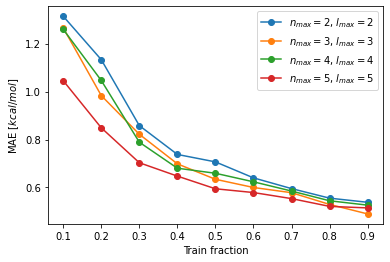
\includegraphics[width=1.0\textwidth]{figures/regression/snap/fixnl.png}
  \endminipage\hfill
  \minipage{0.3333\textwidth}
    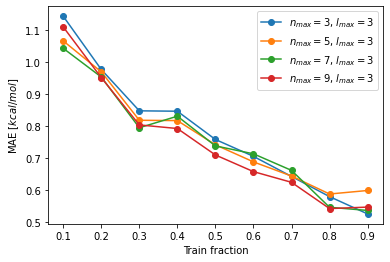
\includegraphics[width=1.0\textwidth]{figures/regression/snap/fixl.png}
  \endminipage\hfill
  \minipage{0.3333\textwidth}
    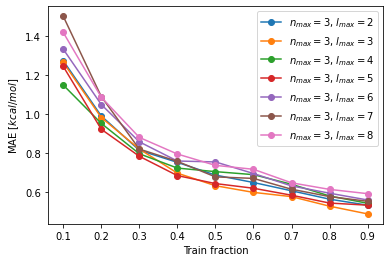
\includegraphics[width=1.0\textwidth]{figures/regression/snap/fixn.png}
  \endminipage
  \caption{
  Networks with specified $n_{max}$ and $l_{max}$ trained on different train fractions.
  All networks were trained on the hyperparameters found for the corresponding $n_{max}$ and $l_{max}$.
  Networks were trained with 20 data augmentation steps and a cutoff radius of $10 \AA$.
  Hyperparameter search was run on a training split of 80\%.
  }
  \label{fig:snap_hyperparameter}
\end{figure}

\paragraph{Cutoff sphere}
All hyperparameter searches were run with with a cutoff radius $r_{cut} = 20 \AA$.
This cutoff sphere is large enough to fully fit every element of the dataset into it.
However, due to the nature of the radial basis functions used, the resolution of atoms 
further away from the center will decrease.
Tests with different cutoff radii were therefore performed.
The tests were run on the network architectures found by hyperparamter optimization.
Since the networks architecture is not fully optimized to the cutoff radii, the prediction accuracies
of the networks were not up the levels found in fully hyperparameter optimized networks.
However the assumption was made that good values for $r_{cut}$ on these not fully optimized architectures 
will also translate to good values under fully hyperparameter optimized networks.
This significantly decreased the number of hyperparameter search needed.
Since hyperparameter search will take multiple days to finish, while networks with know hyperparameters
can be trained in a matter of minutes, this meant a significant speedup.


For every configuration of $n_{max}$ and $l_{max}$, a networks were trained for a variety 
of tests splits and data augmentation steps.
These networks were then evaluated by their performance with respect to the cutoff radius.

Up to a cutoff radius of $10 \AA$, the mean network performance improved. %TODO: Rich
At a training fraction of 80\%, the mean classification error among 
all networks decreased from $0.889 \AA$ for a cutoff radius of $5 \AA$ to 
$0.801 \AA$ for a cutoff radius of $10 \AA$.
From there however, increasing the cutoff radius did not improve the accuracy further.
This lead to the hypothesis that atoms closer to the metal center are more important to the activation barrier than atoms further away from the center.
This hypothesis could also explain the slight increase in prediction error when further increasing the cutoff radius.
Since the resolution of the feature space is limited, increasing the cutoff radius might have decreased the accuracy 
with which the inner atoms are described in the features, thus decreasing the prediction accuracy.

To verify this hypothesis, a second experiment was run.
Here, all atoms outside a cutoff sphere were removed from the element before passing it on to the encoder.
The atoms were then encoded with a cutoff radius $2 \AA$ higher than the cutoff sphere to allow for a proper 
encoding of atoms just inside the cutoff sphere.
The networks were once again trained with the hyperparameters found in the initial hyperparameter analysis.
The training was run for cutoff spheres of $2\AA, 4\AA, 6\AA, 10\AA, 15\AA, 20\AA$ resulting in $r_{cut}$ 
of $4\AA, 6\AA, 8\AA, 12\AA, 17\AA, 22\AA$.
For $r_{cut}=4$, no prediction was possible and the networks just predictied the mean of the data.
This was to be expected since at this cutoff radius, only 20\% of the elements are encoded into the features.
However for $r_{cut}=8$ the mean MAE over all networks trained on 80\% of the data was at $MAE = 0.834 \AA$. 
A $r_{cut} = 8$,resulting in a cutoff sphere of $6 \AA$, 96\% of the atoms are included in the data. 
The remaining 4\% fall outside of the cutoff sphere and are therefore ignored. 

For $r_{cut}=12$ the mean MAE over all networks trained on 80\% of the data was at $MAE = 0.836 \AA$. 
A this cutoff radius, 100\% of the atoms are included in the data.
While this accuracy is marginally higher, the difference is so small that is could 
simply be explained by the optimizer falling into different local minima compared to $r_{cut}=8$. 

This lead to the conclusion that, while all atoms in the dataset seem to have an effect on the prediction,
choosing a tight $r_{cut}$ achieves the best prediction accuracies.
When looking at the nature of the encoding, this intuition is verified.
Empty space that is indirectly included into the enocoders features.
Since the encoder will try to encode a density of 0 in these regions, the features 
need to include this information, and competing with the relevant information about the element.
From now on, all cutoff radii will therefor be chosen at $r_{cut} = 12 \AA$.

\begin{figure}[!htb]
  \minipage{0.5\textwidth}
    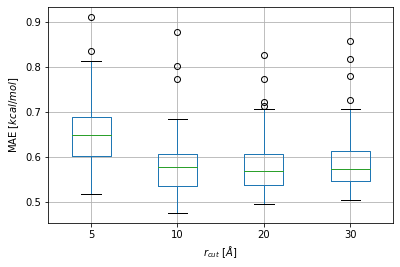
\includegraphics[width=1.0\textwidth]{figures/regression/snap/cut-all.png} %TODO: REPLACE!!!!
  \endminipage\hfill
  \minipage{0.5\textwidth}
    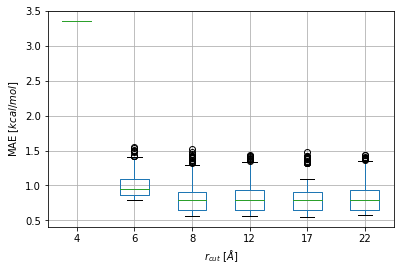
\includegraphics[width=1.0\textwidth]{figures/regression/snap/cut-sphere.png}
  \endminipage\hfill
  \caption{
  Networks trained on different cutoff radii. All networks are trained on a train fraction of 80\%.
  On the left a variety of networks with different $n_{max}, l_{max}$ trained on a test train split of 80\% is shown.
  On the right are networks trained with a cutoff sphere outside of which all atoms are removed. 
  The radius of the cutoff sphere is $r_{cut}-2$.  
 }
  \label{fig:snap_hyperparameter}
\end{figure}


\paragraph{Sensitivity to rotation}
Since snap features are not fully rotationally invariant, the networks ability to abstract rotation from the input is crucial.
In order to teach the network about the possible rotations of an element, 
the element is augmented by rotating it around the remaining axis of freedom, the $z$ axis.
For every augmentation step, the rotated element is added to the training data.
Tests with different augmentation steps were performed.
All networks were trained on the previously found hyperparameters.
The augmentation steps ranged from 5 evenly spaced rotations to 100 evenly spaced rotations.
Both the training and the test data was augmented to allow for learning from the augmented data
as well as to validate if the network was actually able to abstract away rotations.

Even with only 5 data augmentation steps the networks achieved a mean prediction error of $MAE = 40 \AA$.
The mean error over all networks decreased up to 40 augmentation steps.
After 40 augmentation steps no further decrease in mean prediction error was observed ~\ref{fig:snap_roation_out}.
For networks with higher data augmentation steps, the stability of the networks when trained on small train splits was higher.

When looking a networks prediction over 360 different rotations, networks trained with higher data augmentation 
are significantly more stable to rotation than networks trained on a smaller number of of rotations \ref{fig:snap_roation}.
When comparing a network trained on 20 rotations to a network trained on just 5 rotations,
the difference becomes clear.
For the network trained on 5 rotations, for samples from the training data the prediction is very precise 
for the 5 augmentation steps that were part of the training data, but diverges strongly in between the steps from the training data.

For the network trained on 20 rotations, the divergence is very limited.
However in some cases, while the overall prediction accuracy is increased for the network trained on 
more data augmentations, the accuracy for some rotations is more precise on the network trained on a lower number of augmentations.
Since there is no way of knowing which rotation is the one with the closest to real prediction, in 
a real world application therefor the network trained on a higher data augmentation size is prefreable.

Between a augmentation size of 20 to 30, the networks ability to better abstract away rotation is stagnant.
Augmenting the data by 20 to 30 steps therefor seems sufficient to teach the network about all possible rotations.
Interestingly, for some networks while the ability to abstract away rotation no longer increases after 20 augmentation 
steps, the overall performance increases slightly, especially for small training splits.

One hypothesis here would be that the higher number of training data that comes with a bigger number of data augmentations
helps the network to learn about the general structure of catalyst molecules.
While the different rotations of the molecule do not include any new data, the still contain the 
general shape of a catalyst, that might help the network learn about the general topology of the input data.
The might be a hint that transfer learning with an enhanced dataset might be an option to further increase
the prediction accuracy.
In further iterations the test error might be improved by creating a second dataset with a variety of different catalysts molecules.
Due to the combinatorial approach in which molecules surrounding Vaska's complex can be generated, 
creating datasets with a large number catalyst molecules is relatively simple.
The problem comes with calculating their activation barrier.
The key advantage of a transfer learning approach to pre-train the model is that the activation barrier of the extended dataset does not have to be computed.
Instead, properties related to the activation barrier that can be easily computed from the molecules structure are generated.
In a first step, the network would then be taught to predict these east to compute features.

In a second step, the networks topology would be slightly adapted to perform single values regression.
However, the weights and biases will not be changed.
The network is then trained again on the small dataset for which the activation barrier is known.

This approach might help the network to gain more knowledge about the general structure of a catalyst molecule,
and thus reduce overfitting.
The hope is that with this approach the prediction accuracy will improve again.

If this hypothesis holds true will have to be explored in further experiments.


\begin{figure}[!htb]
  \minipage{0.3333\textwidth}
    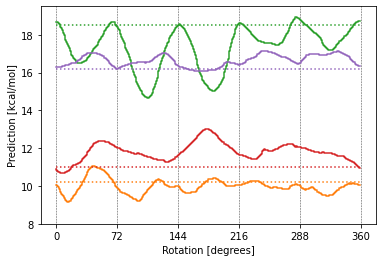
\includegraphics[width=1.0\textwidth]{figures/regression/snap/aug-5steps-30per.png}
  \endminipage\hfill
  \minipage{0.3333\textwidth}
  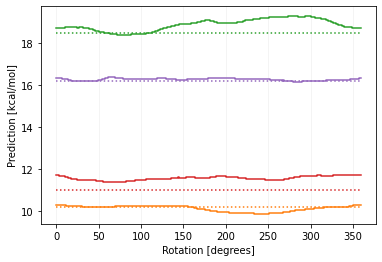
\includegraphics[width=1.0\textwidth]{figures/regression/snap/aug-30steps-30per.png}
  \endminipage\hfill  
  \minipage{0.3333\textwidth}
    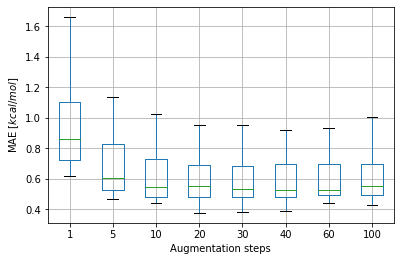
\includegraphics[width=1.0\textwidth]{figures/regression/snap/augmentation.png}
  \endminipage\hfill
  \caption{
  The predictions for a network on SNAP features for $n_{max}=9, l_{max}=3$ trained with 5 data augmentation steps (left) 
  and 20 augmentation steps (middle) for 4 randomly selected samples. 
  The continuos line is the prediction of the network, the dotted line is the calculated barrier.
  The networks were trained on a train split of 70\%.
  On the right are the results for multiple models trained on different augmentation steps.
  All networks are trained on the same network architecture, at different train fractions.
  }
  \label{fig:snap_roation}

\end{figure}


\paragraph{Results}

With the data learned from the extensive hyperparameter and input space exploration, a final hyperparameter
optimization was performed.
This hyperparameter optimization took into account the values discussed previously, and therefore was run on 
features  generated with $n_{max} = 9, l_{max} = 3, r_{cut}=12$.
30 data augmentation steps were passed to the hyperparameter optimizer.
For train fractions from 10\% to 90\% 9 separate hyperparameter optimizations were run 
to ensure the optimal network architecture for each of the test splits.

%TODO Disscuss differences in network achrichtectues

Even with slight variations in prediction accuracy due to rotations, the overall results of regression performed on SNAP features is still promising.
All models found during hyperparameter optimization for different $n_{max}, l_{max}$ were able to predict the reaction barrier with higher accuracies in the
range of the best models found so far.
With the best models for $l_{max}=n_{max}=8$ achieving accuracies of $MAE=0.435 kcal/mol$ and $r^2=0.978$. %TODO: Verbessern

The best network found for a train fraction of 80\% after manual adjustment of the hyperparameters was at $n_{max}=l_{max}=3$. %TODO: Verbessern
It achieved an accuracy of $MAE=0.376 kcal/mol$ and $r^2=0.980$ on a train split of 80\%. %TODO: Verbessern
%TODO: Verbessern
The network used a total of 3 hidden fully connected layers, with an increasing number of neurons.
BatchNormalization and dropout layers were used between the fully connected layers.
Their placement was determined by the hyperparameter optimizer.

Compared to other modes of encoding the data, SNAP seems to be especially susceptible to outliers.
For all models, the regression accuracy is heavily influenced by a small number of samples with poor precision.
Since the split between training and test data is random, the overall accuracy of the model is 
heavily influenced by the selection of samples in the test data.
The same holds true for the randomness between training and validation data.

Improving the networks stability to outliers could further increase regression accuracy.


\section{Comparison}
\label{sec:Evaluation:Comparison}

The neural networks proposed here were able to predict the activation barriers with high accuracies.
The reference values to the networks was given by \cite{friederich_dos}, where different Machine Learning 
approaches to the regression problem were introduced.
While the dataset was the same in \cite{friederich_dos}, the features extracted from the molecules were different.
The comparison of the results from \citetitle*{friederich_dos} and this thesis is therefor more 
a comparison of feature extractors, and not a comparison of machine learning methods or network architectures.

Their best neural network trained on 80\% of the data achieved a prediction accuracy of $MAE = 1.12 kcal/mol$ and a 
coefficient of determination of $r^2 = 0.845$.
The neural network was 4 layers deep and trained on their autocorrelation features.
Autocorrelation features extract features from a graph representation of the chemical structure, but neglect the 
3d structure of the molecule \cite{friederich_dos}.
The best prediction accuracy was however in a yet unreleased paper by  a graph convolution neural network (GNN) on 
a graph structure of the molecule.
It achieved an accuracy of $MAE = 0.571 kcal/mol$ and $r^2=0.964$.
These are the highest accuracies achieved on this dataset yet.
While this was the state-of-the-art  to compare the models in this thesis to, the main objective was not to beat these numbers.
The goal was rather to achieve similar performance with a feature descriptor that allowed for a mapping back from feature space to 3d space.
This allows for an extensive interpretation of the results, which is impossible with current features.
The SNAP features however not only allow for this analysis, but are also able to beat the accuracy of GNN models.
Another important metric is the performance of the networks for different sizes of training data.
The models performance will therefore be compared by their accuracy for different test split sizes.
\\
The first approach regression was using LEFD features.
When training on 80\% of LEFD features, the best neural network achieved an accuracy of $MAE = 1.096 kcal/mol$ and $r^2=0.882$.
While the accuracy is slightly higher than the best neural network in \cite{friederich_dos}, it still falls short 
of the GNN.
Interestingly, the accuracy of the model is very similar to the accuracy achieved by the neural network trained on autocorrelation 
features.
Additionally the autocorrelation features could be approximated from the LEFD features reasonably well.
This could indicate that LEFD features and autocorrelation features describe
similar information about the element that is relevant to the activation barrier.
\\
The best models trained on SNAP features were able to achieve accuracies well below the $0.5 kcal/mol$ barrier.
While the final accuracies are heavily dominated by outliers, models trained on SNAP features were consistently
able to achieve accuracies better than the best model so far.
Another interesting property of models trained on SNAP is their ability to perform well with small amounts 
of training data.
Even with training fractions well below 50\% of the data, the network still achieved good accuracies.
This could be partly due to the fact that the hyperparameter optimization was run for each split separately,
ensuring a good fit of the model architecture to all the data in the training set.
However even when training a network architecture found for a different test split, the 
prediction accuracy still scales significantly better than other prediction methods.

The biggest problem with SNAP features so far seems to be their sensitivity to outliers.
While the majority of the elements in the dataset is predicted with very high accuracy, 
there are some outlier with very poor performance.
Depending on the application of the network, a network with a lower overall accuracy 
that is less susceptible to outliers might be preferred.


\section{Explaining the prediction}

Traditionally neural networks are seen as a black-box approach to data analysis.
The network is given a set of training data and trained to fit onto the data,
the internals of the network however are set by the optimization algorithm.

This makes it hard to interpret the origin of predictions of the network.
Network explaining methods aim to help to understand the origin of a prediction in the features.
Translating the features back into chemical space can help to better understand 
the elements in the dataset and might give intuitions on how elements have to be adapted in order to change their activation barrier.

Since SNAP features achieved significantly higher prediction accuracies,
this analysis was focused on SNAP features only.

\subsection{SHAP}

The first approach to explaining the feature space was using the SHAP feature explainer.
SHAP offers analysis of the influence of different features to the final prediction \cite{NIPS2017_7062}.
This allows get an intuition on how different species influence the activation barrier.

When using SHAP values on our model, we will be able to tell which feature contributes to the current prediction.
The values generated by SHAP are a matrix the sitze of the input to the network.
Summing over all SHAP values for one sample will give us the prediction of that sample.
When labels for the features are  known, SHAP is often visualized as as features pushing in opposite direction with different force 
to achieve the prediction of the model.
In the case of unlabeled input matrices, we can visualized SHAP as positive for each one of out features.
The SHAP values will not correspond to the activation barrier directly,
but rather to the scaled activation barrier we used to train our network.

Scaling issues also make the interpretation of the SHAP values vary hard.
If we think back to the main objectives of SNAP, being able to convert the features back into 
a 3D density was one of the key points.
While we could use the formula describing the density space to transform the SHAP values 
into a 3D density, it is unclear how the density generated by SHAP would have to be interpreted.

Due to the nature of the SNAP encoder, a negative $c_{nlm}^Z$ values does not automatically 
describe a negative density.
This means a negative SHAP values for an element does not equate reduction in density
at a point in space.
In order to get information about the 3D space surrounding the atom, we'd have to convert back from 
the SHAP values to density space.
However here we run into the problem that SHAP values try to predict the output
of an element, and therefor are in the scale of the output.
If we were to convert SHAP values back to 3D, it is unclear how these scaling issues would 
affect the result. 
This uncertainty also prohibits a interpretation of the density space.

The information we can extract from SHAP therefor is limited to feature space.

In the case of Figure~\ref{fig:shap}, we can see that the features corresponding to bromine and arsenic seem to decrease the barrier.
Interestingly the features encoding the absence of phosphorus seem to increase the barrier.
The hypothesis here is that adding phosphorus to the element might help to reduce
the barrier.
If this holds true will have to be confirmed in further experiments.

A good sign that the values have some validity is that Iridium never influences the barrier.
Since iridium is present exactly once in all elements, it should not carry any information about the barrier,
and therefore not influence the prediction at all.

SHAP allows us to get some first intuition of the element and how it is atoms influence the barrier.
However, the information we can gain is limited to a global representation of the element.

Examining the density space for it's influence on the prediction is only possible if the scaling
issues can be solved.
Since the scaling issues did not seem to be easily solvable, a second attempt to explain the origin of the prediction
was run using a gradient based method.

\begin{figure}
    \centering
    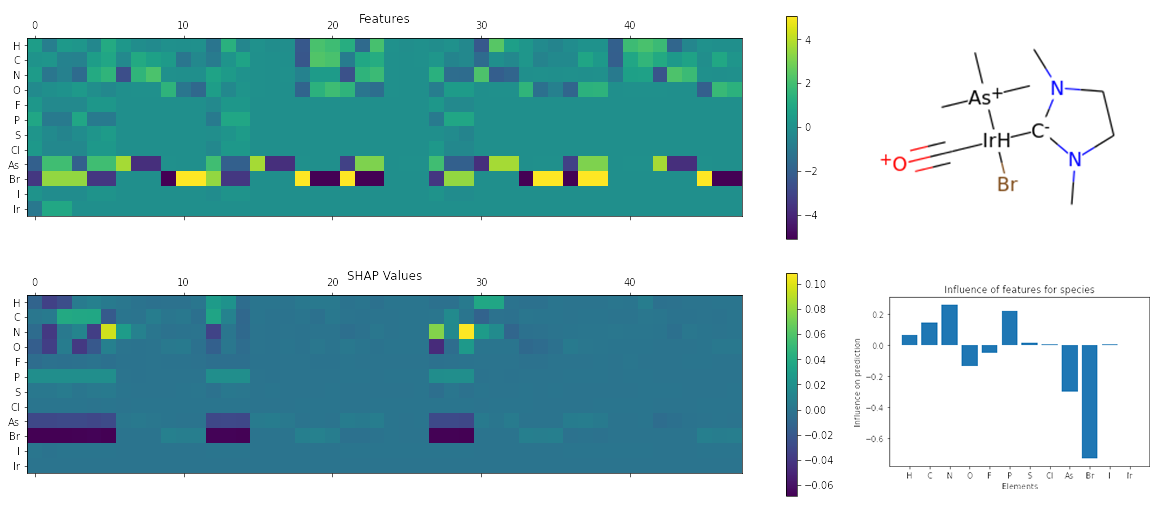
\includegraphics[width=0.9\textwidth]{figures/evaluation/SHAP.png}
    \caption{
        Features($n_{max}=l_{max=3}, r_{cut}=12$) generated by the element on the right and the corresponding SHAP values.
        The element has a calculated barrier of $10.2 kcal/mol$.
        Because the activation barriers are scaled to achieve higher prediction accuracies,
        the values our network predicts is $-0.494$ which scaled back results in a predicted activation 
        barrier of $9.83 kcal/mol$.
     }
    \label{fig:shap}
  \end{figure}
  

\subsection{Gradient explainer}

The information we want to gain from the network is an intuition on
how an element has to be changed in order to lower it's activation barrier.

Let the model $N$ be a function from feature space $\mathbb{R}^n =: \mathbb{S}$ to the activation barrier of the element $\mathbb{R}^+_0$.
Since we can also define a function from density space $\mathbb{D}$ to feature space $\mathbb{S}$,
we can define a mapping from density space to the activation barrier.
$$ \Psi : \mathbb{D} \to \mathbb{S} \to \mathbb{R}^+_0, e \mapsto \Psi(e) $$

While this mapping is only an approximation, the previous chapters show that the 
the accuracy of this approximation is very high.

Looking at the derivative of $\Psi$, we get the gradient $\nabla \Psi$ that points in towards the steepest ascent.

If $\mathbb{D} \to \mathbb{S}$ was a perfect bi-directional mapping, in theory we could follow the gradient until we reach 
a local minima, an then translate back to density space.
This would mean finding a element with similar properties but a lower activation barrier.
This theoretical approach is not possible in practice.
The first problem is the networks lack of understanding of the chemical space.
A simple gradient-decent approach will therefore quickly result in illegal configurations 
that are physically not possible.
The second problem is the low resolution of the feature space.
As shown before, in many cases the density encoding a single atom will not correspond perfectly to the location of this atom.
This problem becomes even more severe when multiple atoms for one species need to be encoded.
This means a perfect translation back from the features is not possible most of the time.

Due to the limited resolution, looking at the gradient itself is more valuable.
Instead of performing a gradient descent approach, we will look at the gradient for a single sample,
and try to gain intuition for the gradient at this datapoint.
When looking at the gradient, it is expected that molecules known to increase the barrier will generate a high density in the gradient.
MOlecules known to decrease the barrier should generate a sub-zero density.
This would indicate that removing elements generating a high density will decrease the barrier,
while removing elements creating a negative density will increase the barrier.

Since the gradient is determined by calculating the derivative of the the network $N$ with input $c$ in respect to the output $N(c): \mathbb{R^N} \to \mathbb{R}$
the gradient vector gives us the direction of steepest ascent for a single sample.
$$
\nabla N: \mathbb{R}^n  \to \mathbb{R}^n 
$$

Since the gradient vector is the derivative of the $c_{nlm}^Z$ coefficients, 
directly interpreting the gradient is challenging. 
Due to the nature of the SNAP encoding, negative $c_{nlm}^Z$ coefficients do not necessarily correlate to negative densities and vice versa.

Instead, we look at the difference in density when adding the gradient to the original features.
Let $f \in \mathbb{S}$ be the feature vector generated by a sample, and $g = \nabla N(f)$ its gradient.

If we think back to the SOAP descriptor, we can now compute the density $\rho^Z(r)$ for $f$ and $f + g$.
The difference between these two densities should give us information about where in space density has negative or positive effects on our prediction.

$$ \rho^Z_\nabla = \rho^Z_{f+g} -  \rho^Z_{f} $$

This gives a 3d dimensional density space in which we can perform interpretations of the result. %TODO: Add figure with n_max=9, l_max=3
Here we encounter the encoding limitations introduced earlier.
While for some atoms, the encoding seems to work as expected, producing regions of negative density where we expect
an increase in the activation barrier, for others the distribution is not precise enough for detailed analysis.
In general, the detail of the encoding does not seem high enough for localized spacial interpretation of the gradient.
Possible solutions to the resolution problem would be to dramatically increase the number of coefficients used to describe a single sample.
This comes with it's own set of challenges, since the size of the features does not scale linear, but rather in $\mathcal{O}(n_{max} \cdot {l_{max}}^3)$.
The cubic scale of $l_{max}$ implies a dramatic increase in the size of the training data, increasing computation time for booth feature generation and training of the regression model.

While the local encoding does not seem the be accurate enough for detailed interpretation,
when integrating over the entire density space, we can get a global influnce for each species.
The output looks similar to what was achieved with SHAP values, but in this case it should allow us to interpret
the influence of the density of a species, rather than just the influence of the features of this species.
This means a high density of one species should indicate that adding more density of this species will increase the barrier.
Similarly, a low density should indicate indicate that adding more density for this species will decreased the barrier.

When looking at the integration over $\rho^Z_\nabla$, we can see it is heavily dominated by hydrogen and carbon
in many cases.
This contradicts the hypothesis on which species should mostly influence the activation barrier.
Here the assumption was that hydrogen and carbon are more "filler-elements", and the activation 
barrier is dominated other atoms.
%TODO: Add figure
It is unclear if the the chemical interpretation here should be that hydrogen and carbon play a bigger role in the activation
barrier than what was expected, ot if this is an artifact of the neural network, an does not actually translate back into 
the physical world.